\chapter{Symbolic Security Analysis Using Scyther}
\label{chp:scyther} 

%Introduction to Scyther. What it is. How it works. Examples.

There exists multiple state-of-the-art tools for performing formal analysis of security protocols, for example Avispa \cite{avispa}, ProVerif \cite{proverif}, and Scyther \cite{scyther}. This thesis uses Scyther as its tool for conducting formal security analysis, and the following chapter will give an introduction to Scyther, how it works, and examples of usages.


\section{The Scyther Tool: Verification, Falsification, and Analysis of Security Protocols}

Scyther is a tool for verification, falsification, and analysis of security protocols developed by Cas Cremers. The tool is based on a patter refinement algorithm that enables unbounded verification, falsification, will also enabling the tool to perform characterization \cite{cremers2008scyther} on the protocol. Scyther allows its users to verify security protocols in two different ways. The first option is to execute Scyther scripts through the command-line interface, which provides an output file containing the results of the protocol verification. Option two, is to use Scyther's own \gls{gui}, which provides panels for both verification results, and in case of attacks being found; a visual graph of Scyther's proposed attack on the protocol. The most recent release of Scyther was published on April 4, 2014, and is currently available for Windows, OS X and Linux.

% Ok

Security protocol specifications are built up of messages that are sent between different entities and computation that is done at either side. Much like a blueprint, these specifications define what a protocol is allowed to do, and how it is allowed to communicate \cite{cremers2003defining}. The blueprint can then be modelled using Scyther, where the entities are converted into roles, the messages are converted into send and receive events, and the security requirements into claim events. Scyther performs complete characterization of a protocol, where roles are broken down to a finite set of representative behaviours by analysing all the possible execution traces where the events hold. The intuitive idea behind this algorithm is that the set of execution traces together represents all possible ways in which the protocol could execute, and grouping them into patterns which are partially ordered, symbolic set of events  \cite{cremers2006scyther}. From the patterns, Scyther is able to construct a complete set of attack traces for each security claim. When analysing protocols, the realizable traces are compared to the attack traces. If none of these realizable traces of the protocol exhibits an attack trace, then there exists no attack, and the security property is verified. 

Most protocols can be characterized into a finite set of traces, which enables Scyther to perform \emph{unbounded} verification of the protocol. This greatly differs from the majority of other verification tools which perform \emph{bounded} verification \cite{cremers2008scyther} \cite{cremers2009comparing}. When performing bounded verification, there exists a finite set of traces that the tool is able to verify, meaning that the entire space of possible states is not covered in the verification process \cite{cremers2008unbounded}. At best, such a verification can guarantee that the security requirements hold under a finite subset of the actual state-space. Unbounded verification, however, is to verify all possible states, or behaviours, of the protocol which is a great enhancement compared to bounded verification algorithms. In addition to handling an infinite state-space, Scyther's algorithm is also guaranteed to terminate, which gives it the ability to provide useful results even when it is not able to establish unbounded correctness, or in the scenario of where no attack is found.

As mentioned, a protocol specification contains a set of roles which serves as blueprints that describes what the protocol is able to do. When executing the protocol, each of the different roles can be executed multiple times, and in parallel with each other by one or more agents \cite{cremers2006scyther}. An execution of a role is referred to as a \emph{run}, and defines an unique instance of the protocol with respect to local constraints and the binding between the role and the actual agent acting out the roles behaviour. Scyther allows its users to state security claims which are evaluated as they appear in the protocol trace, either ending in a successful verification of the security property, or in a failure. In the presence of a failure for some security property, Scyther will provide a concrete attack on the protocol by utilizing one of the attack traces from the pattern, and it will also present an attack graph to easier illustrate the  threat. If the protocol developer is unsure of what types of claims that should be stated for each role, Scyther has support for so-called verification of automatic claims, where Scyther will provide the appropriate claims for each variable or key based on its type.

Another of the major novelties in Scyther is the possibility for performing so-called multi-protocol analysis, which in short terms is to analyse multiple protocols that are co-existing in the environment. Such an analysis has previously been infeasible because of an incredible wide state-space, but thanks to Scyther's unique algorithm that operates on an unbounded state-space, it allows for conducting multi-protocol analysis. 


\section{Scyther Syntax}


The syntax used in \verb!.spdl!-files, which are protocol files that can be run and verified by Scyther, can resemble popular object-oriented languages such as C, C++ or Java. Below is the structure of a minimum working example of the protocol known as \gls{apkes}, consisting of an outer class defining the protocol and multiple agents (or roles) inside the protocol. In this example, we define that our protocol consists of two communicating parties; U and V, without giving them any specific behaviour.\newline

\begin{lstlisting}
protocol APKES(U, V){
	role U { };
	role V { };  
};
\end{lstlisting}

For each of the different roles in the protocol, behaviour can be added as a sequence of send and receive events, as well as variable declarations, constants and claims. For the U role, we can define a simple behaviour as shown below, where U generates a random nonce \texttt{Ru} and sends it to V, before receiving a message from V containing the random nonces \texttt{Ru} and \texttt{Rv}. All events are labelled with either \texttt{send} or \texttt{recv} followed by a subscript and a number. The number indicates the message's position in a \gls{msc}, and must be incremented for each message sent.\newline

\begin{lstlisting}
role U{
	fresh Ru: Nonce; # Freshly generated nonce
	var Rv: Nonce; # Variable for receiving a nonce
	
	send_1(U, V, Ru); # Send message to V containing Ru
	recv_2(V, U, Ru, Rv); # Receive message from V containing Ru and Rv. Store Rv in variable
};
\end{lstlisting}



Typically, a \texttt{send}-event has a corresponding \texttt{recv}-event at the receiving role with the same number.\newline


\begin{lstlisting}
role V{
	[...]
	
	recv_1(U, V, Ru); # Receive message sent from U containing Ru. Store Ru in variable
	send_2(V, U, Ru, Rv); # Send message to U containing Ru and Rv
};
\end{lstlisting}


Along with support for creating fresh nonces, variables, and terms, Scyther also provides a wide set of cryptographic elements such as hash functions, symmetric-key cryptography, public-key cryptography, as well as declaring user specific types and macros, which are abbreviations of complex expressions into simpler once. In the following example, a hash function is used to define a function that generates a \gls{mic} (which is essentially the same as a \gls{mac-auth}). On the next line, we have created a macro representing the generation of a pairwise key between U and V. The key is represented as an encryption of the two values \texttt{Ru} and \texttt{Rv} using a symmetric key that is shared between U and V. Constants and functions defined outside of a role are considered to be global, and available to all of the defined roles in the protocol.\newline

\begin{lstlisting}
hashfunction MIC; # An hashfunction to represent a Message Integrity Code (MIC) generation.

macro PairwiseKey = {Ru, Rv}k(U, V);


role U {


}
\end{lstlisting}


\subsection{Security Claims}

A sequence of events within a role is usually followed by a set of claim events. Claim events are used for describing security properties of a role, for example that some value should be considered secret, or that certain properties hold for authentication. Such claims can be formally verified using Scyther. If the protocol is not instructed with any security claims, Scyther is able to generate the appropriate claims  for the protocol with respect to secrecy and authentication by using the ``Verify automatic claims'' alternative provided by the \gls{gui}.

\subsubsection{Secret}

The first, most trivial security claim is secrecy. Secrecy expresses that the stated property is to be kept hidden from an adversary, even in the case of where the adversary controls the network used for communication. However, if one of the agents gets compromised by the adversary and the protocol is executed between an honest agent and the adversary, it would in the end learn what was meant to be kept hidden from it \cite{cremers2005operational}. The secrecy claim does not hold for such cases (nor is it intended to), but for each case where the protocol is executed between two honest agent where the secret property is successfully kept hidden from the adversary. For our example protocol, we can claim that the two values \texttt{Ru} and \texttt{Rv} are supposed to be secret and thereby hidden from the adversary as shown below. These claims will obviously fail as we have not specified that any encryption should be used on the messages that are passed between the two roles.\newline

\begin{lstlisting}
role U{
	[...]
	
	# Claims:
	claim_F1(U, Secret, Ru);
	claim_F2(U, Secret, Rv);
};
\end{lstlisting}




\subsubsection{\gls{skr}}

Session keys are created at the end of a key establishment process, and are usually used for a session of the communication, before being replaced. When they expire, they are deleted from the system and never used again, limiting the amount of ciphertexts available for the adversary to perform cryptanalysis. In Scyther, the claim \gls{skr} is used to identify the session keys in the protocol, and claim that they are secret. For the \gls{skr} claim to function correctly, Scyther's session-key reveal checkbox needs to be checked in the settings. With this setting enabled, Scyther will reveal any session-key, whose run identifier differs from the current session's, to the adversary. If the \gls{skr} claim is used without enabling the setting, the claim is verified as a regular secret claim as defined by Scyther. 

%\gls{skr} is mostly the same as the regular secrecy claim, but is used to highlight that the term that is claimed to be secret is also a session key. This instructs Scyther to reveal the session key to the adversary after it has executed its run, hence proving that the session keys are working correctly, and that current session keys are kept secret from the adversary \cite{scyther-manual}.  If not, this claim is identical to the ordinary secrecy claim presented above.



\subsubsection{Aliveness}

Aliveness is considered to be the weakest form of authentication, guaranteeing to the initiator of a protocol (U) that if it completes a run successfully, then the intended responder (V) of the run has previously executed the protocol \cite{lowe1997hierarchy}. This does not necessarily mean that V knew that he was interacting with U, nor does it mean that it has executed the protocol any time recently. 


\subsubsection{Weak Agreement}

Weak agreement strengthens the authentication form introduced as aliveness. Such an authentication states that the responder in fact was executing the protocol with the initiator (U), and not just having run the protocol at some point in time \cite{lowe1997hierarchy}. By claiming that the protocol holds under the weak agreement, we state that if U successfully completes a run with the intended responder (V), then V confirms that it has previously run the protocol with U. Such a claim would prevent an adversary from acting as a responder by running another run of the protocol in parallel with a run with U, and conducting a man-in-the-middle-attack. The Needham-Schroeder case presented in Chapter \ref{chp:background} failed on this claim, allowing Lowe to construct his attack. 


\subsubsection{Non-injective Agreement}

Where the authentication provided by weak agreement does not specify which of the two communicating parties acted as initiator and responder, non-injective agreement does. It guarantees that if the initiator (U) successfully completes a run of the protocol, apparently with the responder (V), then V has completed a run with U, where he acted as a responder \cite{lowe1997hierarchy}. This does, however, not indicate that they both have executed exactly one run. There is still a possibility that U has executed multiple runs with a responder which he believed to be V, but may in fact have been communicating with the adversary. Another guarantee provided by non-injective agreement is that if U also sends a set of variables to V in the completed run, then they both agree that the data values correspond to all in the sent set of variables.

% Last sentence seems.. weird and stupid and I hate it.

Below is the example protocol claiming that V is in fact alive, has run the protocol at some time with U, and that during this particular run, it was U and V that was communicating.\newline

\begin{lstlisting}
role U{
	[...]
	
	# Claims:
	claim_U1(U, Alive);
	claim_U2(U, Weakagree);
	claim_U3(U, Niagree);
};
\end{lstlisting} 


\subsubsection{Non-injective Synchronization}

Synchronization requires that all protocol messages occur in the expected order with their expected values, and that the behaviour is equivalent to as if the protocol was executed without the presence of any adversary \cite{cremers2006injective}. An injective synchronization property states that the protocol executes as expected over \emph{multiple} runs, claiming that it is not possible for an attacker to use information from previous runs into disrupting the current protocol execution \cite{cremers2005operational}. Such an attack is known as a replay attack, and is used by an adversary to inject traffic into the protocol execution to induce undesirable or unexpected behaviour. Scyther, however, does not support this enhanced form of synchronization, hence it strongest type of synchronization is non-injective synchronization. Because of this, Scyther is not able to verify whether or not a protocol is secure against replay attacks.\newline

\begin{lstlisting}
role U {
	[...]

	# Claims:	
	[...]
	
	claim_U4(U, Nisynch);
}


\end{lstlisting}

%Synchronization = Strong form for authentication. Does not protect against replay attacks. Same for Non-injective synchronization.


\subsubsection{Running, Commit}

Running and commit signals can be used as a form of authentication for some variables from a set of terms sent in a message. By using these signals (in Scyther modelled as claims), we can verify that a variable sent from U to V, and then returned to U, has not been changed from its initial value during transmission. From a formal view, this can be seen as non-injective agreement over a set of terms \cite{scyther-manual}.

The expression $claim(V, Running, U, Ru)$ denotes that V is currently executing the protocol with U, and with the nonce $Ru$. In U's case, $claim(U, Commit, V, Ru)$ indicates that the protocol as reached a point where authentication is claimed (U has completed the protocol run with V), where $Ru$ is the variable that it claimed to be exchanged during this part of the run \cite{ryan2001modelling}. Usually, the \emph{commit} claim is stated at the end of the protocol run. For the correctness of the \emph{commit} claim to hold, it requires that the \emph{running} signal is added in the communicating role, and preceding the \emph{commit} claim in the trace.

This pattern is a scheme for authentication properties, but it also allows for expressing authentication for additional information specific to the particular, for example some variable inside the message. Occurrence of a \emph{commit} signal in U's protocol run guarantees that a corresponding \emph{running} signal has previously occurred in V's protocol run, which guarantees that the received message containing $Ru$ must have been transmitted by V \cite{ryan2001modelling}. Below is an example of how we can claim non-injective agreement over a variable, in this case the nonce $Ru$. 
\newline

\begin{lstlisting}
role U{
	[...]
	
	send_1(U, V, Ru);
	
	recv_2(V, U, Ru, Rv);
	
	claim_U5(U, Commit, V, Ru); # Authentication over the term Ru is claimed
};


role V{
	[...]
	
	recv_1(U, V, Ru);
	claim_V6(V, Running, U, Ru); # Claim that V is currently running the protocol with U with the value Ru
	
	
	send_2(V, U, Ru, Rv); 
}
\end{lstlisting}

\section{Scyther's Graphical Interface}


As mentioned, Scyther provides a \gls{gui} for easily understand and assess the security of a protocol. 
If we continue on our example from the section on Scyther's syntax, we now want to verify all the stated security claims. By using the \gls{gui}, we can configure the verification process by providing a maximum number of runs, the adversary compromise model, as well as more advanced options for how to prune the search space. Scyther provides three options in its \gls{gui}; verification of claims, verification of automatic claims, and characterization of the protocol \cite{cremers2008scyther}. Figure \ref{fig:scyther-verify-claims} contains the results of running a verification of the claims previously described for a secure protocol.

\begin{figure}[h]
	\centering
	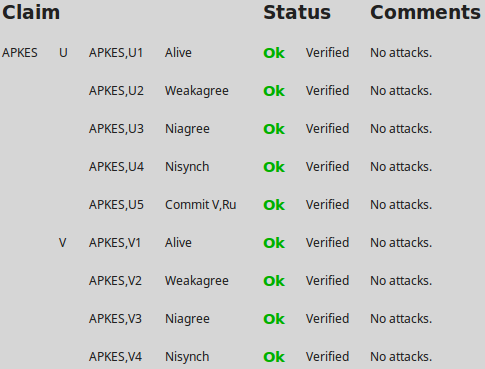
\includegraphics[scale=0.9]{Untitled.png}
	\caption{Results of a verification process using Scyther where all claims are successfully verified.}
	\label{fig:scyther-verify-claims}
\end{figure}


Scyther returns an \texttt{Ok} status code for each claim that is successfully verified. As we see in Figure \ref{fig:scyther-verify-claims}, Scyther is not able to find any attacks on the protocol. To illustrate the case of Scyther actually finding an attack, we try to verify the claims introduced in the section on secrecy, claiming that \texttt{Ru} and \texttt{Rv} are secret. In our example protocol, both nonces are sent in plaintext between U and V, hence this claim will naturally fail as seen in Figure \ref{fig:scyther-verify-claims-fail}.

\begin{figure}[h]
	\centering
	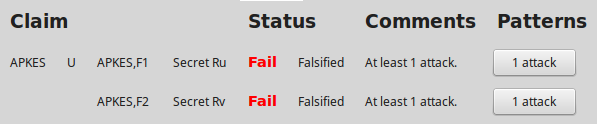
\includegraphics[scale=0.81]{ScytherFailSecretClaim.png}
	\caption{Results of a verification process using Scyther when a claim fails.}
	\label{fig:scyther-verify-claims-fail}
\end{figure}

Whenever Scyther finds an attack on a protocol, it will also provide a concrete description of the attack as graph. An example of such a graph is shown in Figure \ref{fig:scyther-graph}. It contains description of the different runs that Scyther executes, and shows how an adversary can pass messages a cross different runs to learn some secret information for constructing its attack.

\begin{figure}[h]
	\centering
	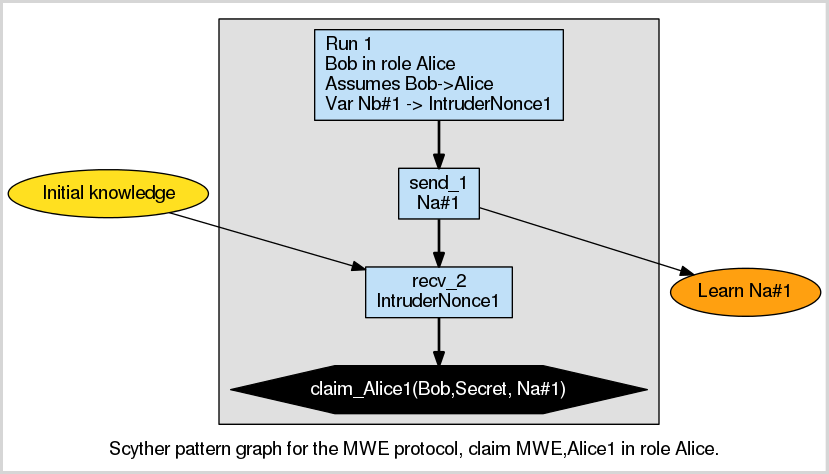
\includegraphics[scale=0.45]{ScytherFailAttackGraph.png}
	\caption{When Scyther finds an attack on a protocol, if will also provide a graph of the attack.}
	\label{fig:scyther-graph}
\end{figure}
